\chapter{Mol dan Massa Molar}\label{ch:g10:the-mole}

Di penghujung hari, sebuah bank tidak menghitung koinnya satu per satu:
bank itu menimbangnya. Jika sekeping koin bermassa \qty{7.5}{g},
sekantong koin bermassa \qty{7.5}{kg} berisi seribu koin, dan
timbanganlah yang telah menghitungnya. Para ahli kimia menghadapi masalah
yang sama dengan \omterm{def:g7:atoms-and-molecules:atom}{atom}, hanya jauh lebih parah: sesendok air mengandung
lebih banyak \omterm{def:g7:atoms-and-molecules:molecule}{molekul} daripada butir pasir di semua pantai sepanjang
sebuah pesisir. Mereka memecahkannya dengan cara yang sama, dengan
menimbang, dan ``kantong'' yang mereka pakai berisi
\num{602214076000000000000000} entitas. Bab ini mendefinisikan kantong
itu, yaitu \omterm{def:g10:the-mole:amount}{mol}, dan menunjukkan cara beralih dari massa di atas neraca
ke banyaknya \omterm{def:g7:atoms-and-molecules:atom}{atom} atau \omterm{def:g7:atoms-and-molecules:molecule}{molekul}.

\begin{recall}
Massa sebuah \omterm{def:g7:atoms-and-molecules:atom}{atom} terpusat di intinya; sebuah \omterm{def:g9:inside-the-atom:proton}{proton} dan sebuah \omterm{def:g9:inside-the-atom:proton}{neutron}
masing-masing bermassa sekitar \qty{1.67e-27}{kg}, sehingga \omterm{def:g7:atoms-and-molecules:atom}{atom} dengan
\omterm{def:g9:inside-the-atom:atomic-number}{nomor massa} $A$ bermassa sekitar $A \times \qty{1.67e-27}{kg}$. Bilangan
yang sangat besar dan sangat kecil ditulis dalam notasi ilmiah
(\cref{ch:g9:inside-the-atom}). \omterm{def:g7:atoms-and-molecules:formula}{Rumus kimia} menyatakan banyaknya \omterm{def:g7:atoms-and-molecules:atom}{atom}
setiap unsur dalam sebuah \omterm{def:g7:atoms-and-molecules:molecule}{molekul} (\cref{ch:g7:atoms-and-molecules}).
\end{recall}

\begin{omfigure}
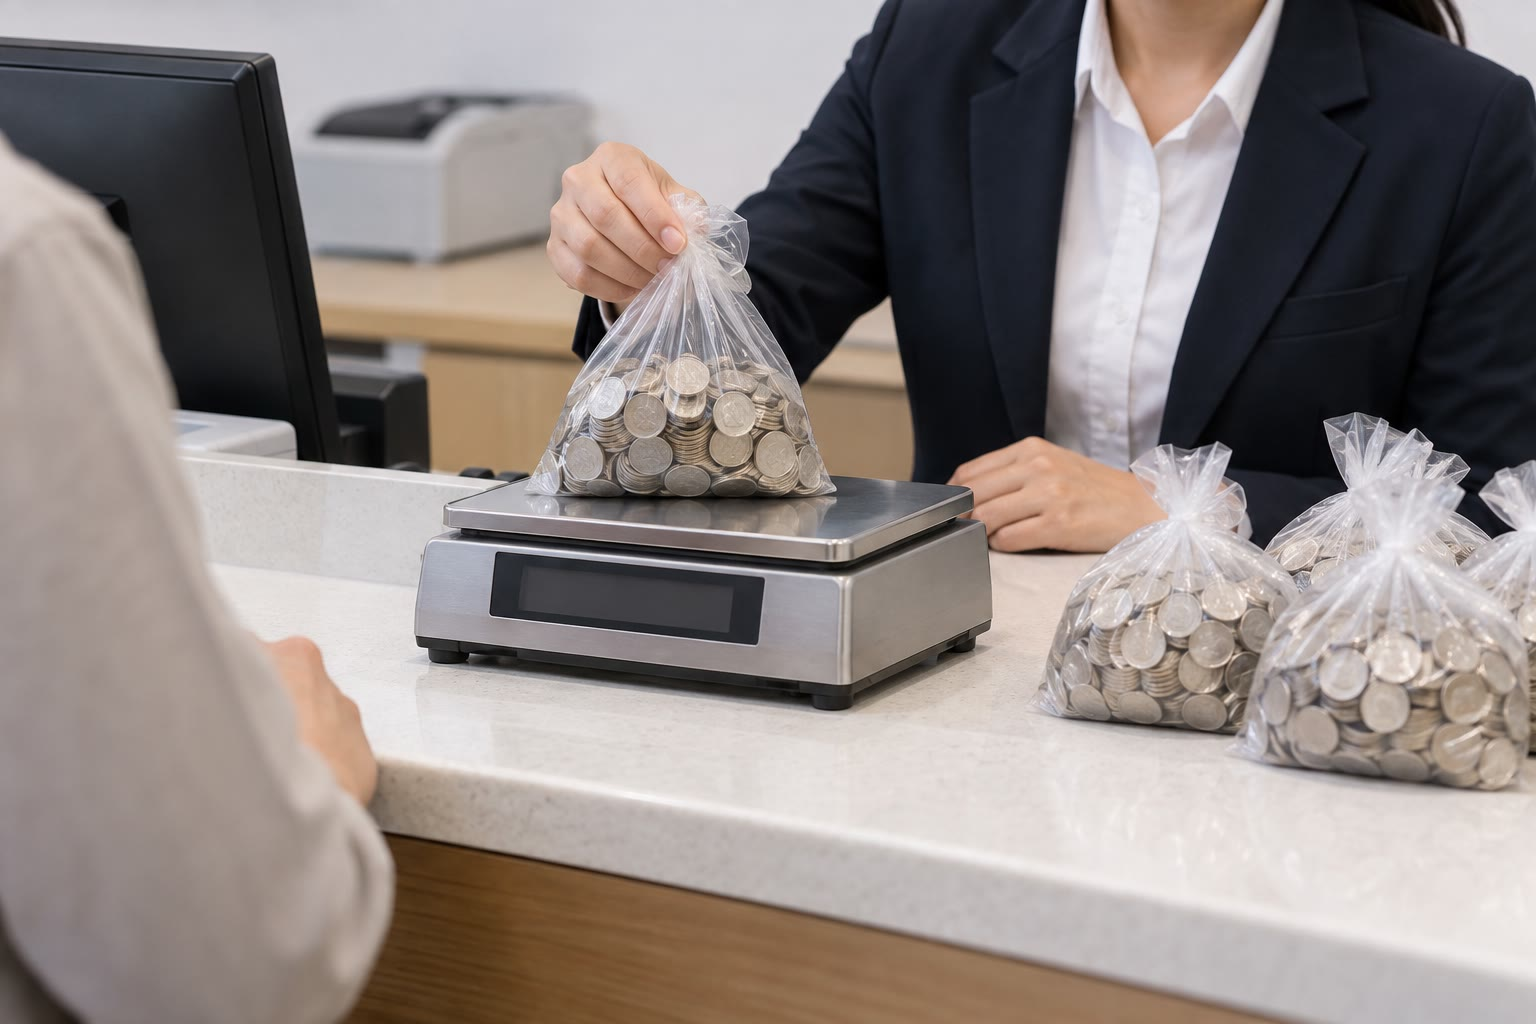
\includegraphics[width=0.55\linewidth]{images/book1/ai/g10-bank-coins.jpg}

{\small Bank menghitung koin dengan menimbangnya. Para ahli kimia
menghitung \omterm{def:g7:atoms-and-molecules:atom}{atom} dengan cara yang sama.}
\end{omfigure}

\section{Menghitung dengan menimbang}

\begin{example}[Sekantong koin]\label{ex:g10:the-mole:coins}
Sekeping koin bermassa \qty{7.5}{g}. Sekantong koin ini bermassa
\qty{1.80}{kg}, yaitu \qty{1800}{g}, tanpa menghitung massa kantongnya.
Kantong itu berisi
\[
  \frac{\qty{1800}{g}}{\qty{7.5}{g}} = 240 \text{ koin.}
\]
Untuk menghitung, bank membagi massa total dengan massa sekeping koin.
\end{example}

\begin{example}[Sesendok air]\label{ex:g10:the-mole:spoon}
Sebuah \omterm{def:g7:atoms-and-molecules:molecule}{molekul} air, \ce{H2O}, memiliki $2 + 16 = 18$ \omterm{def:g9:inside-the-atom:proton}{nukleon} (\omterm{def:g7:atoms-and-molecules:atom}{atom}
oksigen-16 dan hidrogen-1 menyusun hampir seluruh air alami), sehingga
massanya sekitar $18 \times \qty{1.67e-27}{kg} = \qty{3.0e-26}{kg}$,
atau \qty{3.0e-23}{g}. Karena itu sesendok air \qty{5.0}{g} berisi
\[
  \frac{\qty{5.0}{g}}{\qty{3.0e-23}{g}} \approx \num{1.7e23}
  \text{ molekul.}
\]
Pembagian itu bekerja seperti untuk koin, tetapi hasilnya adalah
bilangan yang tidak dapat dibayangkan siapa pun. Para ahli kimia
memerlukan ``bungkusan'' \omterm{def:g7:atoms-and-molecules:atom}{atom} yang sesuai dengan sampel-sampel di
laboratorium.
\end{example}

\begin{definition}[Jumlah zat dan mol]\label{def:g10:the-mole:amount}
% ledger: const:NA
Yang disebut \emph{jumlah zat}\index{jumlah zat} $n$ sebuah sampel
menghitung entitas yang dikandungnya (\omterm{def:g7:atoms-and-molecules:atom}{atom}, \omterm{def:g7:atoms-and-molecules:molecule}{molekul}, atau \omterm{def:g9:ions:ion}{ion}, yang
harus disebutkan setiap kali). Satuannya adalah \emph{mol}\index{mol},
dengan lambang \si{mol}: satu mol mengandung tepat \num{6.02214076e23}
entitas.
\end{definition}

\begin{remark}[Selusin, serim, satu mol]\label{rem:g10:the-mole:dozen}
\omterm{def:g10:the-mole:amount}{Mol} adalah satuan hitungan, seperti selusin telur (12) atau serim kertas
(500 lembar), hanya jauh lebih besar. ``Dua \omterm{def:g10:the-mole:amount}{mol} \omterm{def:g7:atoms-and-molecules:molecule}{molekul} air'' berarti
$2 \times \num{6.02214076e23} = \num{1.20e24}$ \omterm{def:g7:atoms-and-molecules:molecule}{molekul}, sama seperti
``dua lusin telur'' berarti 24 butir telur. Selalu sebutkan entitas apa
yang dihitung: satu \omterm{def:g10:the-mole:amount}{mol} \emph{\omterm{def:g7:atoms-and-molecules:molecule}{molekul}} oksigen \ce{O2} mengandung dua
\omterm{def:g10:the-mole:amount}{mol} \emph{\omterm{def:g7:atoms-and-molecules:atom}{atom}} oksigen.
\end{remark}

\begin{history}[Hipotesis Avogadro, 1811]
Pada tahun 1811 fisikawan Amedeo Avogadro mengusulkan bahwa gas-gas yang
berbeda dengan volume sama, pada suhu dan tekanan yang sama, mengandung
partikel dalam jumlah yang sama. Ia juga memahami bahwa gas seperti
oksigen tersusun atas \omterm{def:g7:atoms-and-molecules:molecule}{molekul-molekul} beratom dua. Gagasannya diabaikan
selama hampir lima puluh tahun, sampai Stanislao Cannizzaro memakainya
pada tahun 1860 untuk memperoleh serangkaian massa \omterm{def:g7:atoms-and-molecules:atom}{atom} relatif yang
taat asas. Tetapan yang menghitung entitas dalam satu \omterm{def:g10:the-mole:amount}{mol} kemudian
dinamai menurut nama Avogadro; ia sendiri tidak pernah mengetahui
nilainya.
\end{history}

\begin{omfigure}
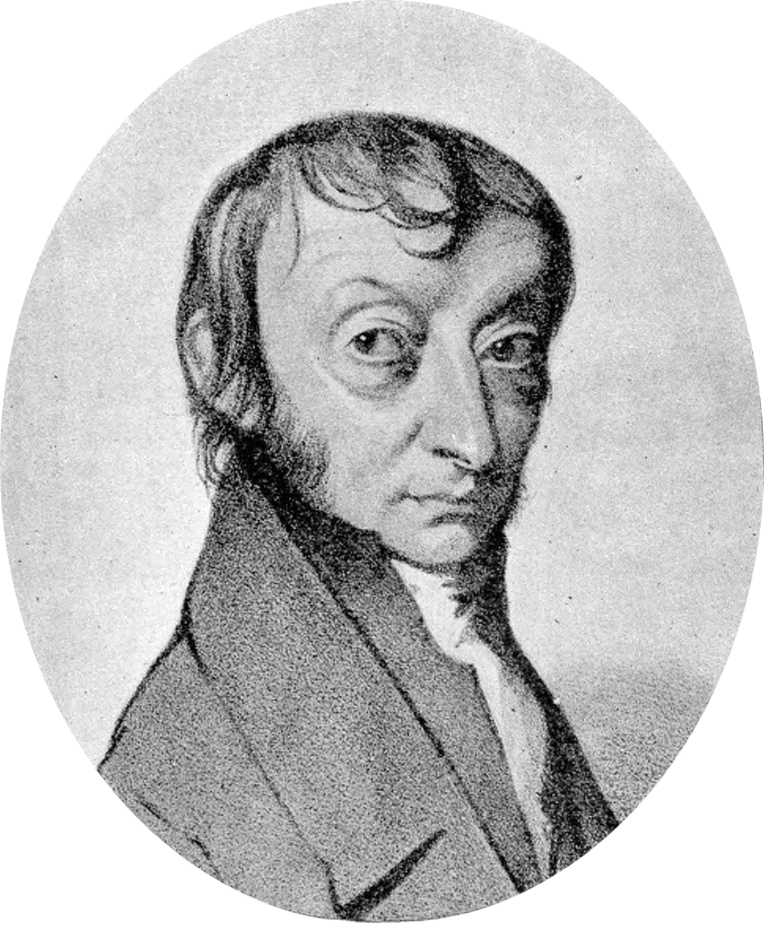
\includegraphics[width=0.26\linewidth]{images/book1/avogadro.jpg}

{\small Amedeo Avogadro (1776--1856).}
\end{omfigure}

\section{Tetapan Avogadro}

\begin{definition}[Tetapan Avogadro]\label{def:g10:the-mole:avogadro}
% ledger: const:NA
Yang disebut \emph{tetapan Avogadro}\index{tetapan Avogadro} $N_A$
adalah banyaknya entitas per \omterm{def:g10:the-mole:amount}{mol}:
\[
  N_A = \qty{6.02214076e23}{mol^{-1}} .
\]
Nilainya eksak, ditetapkan menurut definisi. Dalam perhitungan, nilai
itu dibulatkan menjadi \qty{6.02e23}{mol^{-1}}.
\end{definition}

\begin{proposition}[Banyaknya entitas dan jumlah zat]\label{prop:g10:the-mole:number}
Sebuah sampel yang memuat $N$ entitas mengandung \omterm{def:g10:the-mole:amount}{jumlah zat}
\[
  n = \frac{N}{N_A}, \qquad\text{yaitu}\qquad N = n \times N_A .
\]
\end{proposition}

\begin{proof}
Setiap \omterm{def:g10:the-mole:amount}{mol} mengandung $N_A$ entitas, sehingga $n$ \omterm{def:g10:the-mole:amount}{mol} mengandung
$n \times N_A$ entitas; membaginya dengan $N_A$ menghasilkan $n$.
\end{proof}

\begin{example}[Molekul dan mol]\label{ex:g10:the-mole:convert}
Sebuah sampel mengandung \num{1.5e24} \omterm{def:g7:atoms-and-molecules:molecule}{molekul} karbon dioksida. Jumlah
karbon dioksidanya adalah
$n = \num{1.5e24} / \qty{6.02e23}{mol^{-1}} = \qty{2.5}{mol}$.
Sebaliknya, \qty{0.20}{mol} besi memuat
$N = \qty{0.20}{mol} \times \qty{6.02e23}{mol^{-1}} = \num{1.2e23}$
\omterm{def:g7:atoms-and-molecules:atom}{atom} besi.
\end{example}

\begin{remark}[Asal bilangan itu]\label{rem:g10:the-mole:origin}
Selama lebih dari lima puluh tahun, \omterm{def:g10:the-mole:amount}{mol} didefinisikan sebagai banyaknya
\omterm{def:g7:atoms-and-molecules:atom}{atom} dalam tepat \qty{12}{g} karbon-12, dan $N_A$ harus diukur. Sejak
2019 bilangan itu sendiri telah ditetapkan, sehingga \omterm{def:g10:the-mole:amount}{mol} menjadi hitungan
murni. Definisi lama dan baru sesuai sampai lebih baik daripada satu
bagian per seratus juta, sehingga dua belas gram karbon-12 tetap
mengandung satu \omterm{def:g10:the-mole:amount}{mol} \omterm{def:g7:atoms-and-molecules:atom}{atom}, seperti yang diperiksa pada subbab berikut.
\end{remark}

\section{Massa molar}

\begin{definition}[Massa molar]\label{def:g10:the-mole:molar-mass}
Yang disebut \emph{massa molar}\index{massa molar} $M$ sebuah \omterm{def:g6:pure-substances-and-mixtures:species}{spesies
kimia} adalah massa satu \omterm{def:g10:the-mole:amount}{mol} entitasnya, dalam gram per \omterm{def:g10:the-mole:amount}{mol}
(\si{g/mol}). Massa molar sebuah unsur, yang dihitung atas \omterm{def:g6:pure-substances-and-mixtures:mixture}{campuran}
\omterm{def:g9:inside-the-atom:isotope}{isotop} alaminya, disebut
\emph{massa molar atom}\index{massa molar atom} unsur itu; nilai ini
dicetak dalam \omterm{def:g9:periodic-table-first-look:periodic-table}{tabel periodik}.
\end{definition}

\begin{example}[Satu mol atom karbon]\label{ex:g10:the-mole:carbon}
% ledger: const:NA, const:u
Sebuah \omterm{def:g7:atoms-and-molecules:atom}{atom} karbon-12 bermassa sekitar
$12 \times \qty{1.67e-27}{kg} = \qty{2.00e-26}{kg}$. Satu \omterm{def:g10:the-mole:amount}{mol} \omterm{def:g7:atoms-and-molecules:atom}{atom} itu
bermassa
\[
  \qty{2.00e-26}{kg} \times \num{6.02e23} = \qty{1.20e-2}{kg}
  = \qty{12.0}{g}.
\]
\omterm{def:g10:the-mole:amount}{Mol} dipilih sedemikian rupa sehingga \omterm{def:g10:the-mole:molar-mass}{massa molar} sebuah \omterm{def:g7:atoms-and-molecules:atom}{atom}, dalam gram
per \omterm{def:g10:the-mole:amount}{mol}, mendekati \omterm{def:g9:inside-the-atom:atomic-number}{nomor massanya}: sekitar \qty{1}{g/mol} untuk
hidrogen, \qty{12}{g/mol} untuk karbon, \qty{16}{g/mol} untuk oksigen.
\end{example}

\begin{omfigure}
% ledger: aw:H, aw:C, aw:N, aw:O, aw:Na, aw:Mg, aw:Al, aw:Si, aw:S, aw:Cl, aw:K, aw:Ca, aw:Fe, aw:Cu, aw:Zn, aw:Au (rounded to 0.1)
\begin{tabular}{lcr@{\qquad}lcr}
\hline
unsur & lambang & $M$ (\si{g/mol}) & unsur & lambang & $M$ (\si{g/mol}) \\
\hline
hidrogen  & \ce{H}  & 1.0  & silikon   & \ce{Si} & 28.1 \\
karbon    & \ce{C}  & 12.0 & belerang  & \ce{S}  & 32.1 \\
nitrogen  & \ce{N}  & 14.0 & klorin    & \ce{Cl} & 35.5 \\
oksigen   & \ce{O}  & 16.0 & kalium    & \ce{K}  & 39.1 \\
natrium   & \ce{Na} & 23.0 & kalsium   & \ce{Ca} & 40.1 \\
magnesium & \ce{Mg} & 24.3 & besi      & \ce{Fe} & 55.8 \\
aluminium & \ce{Al} & 27.0 & tembaga   & \ce{Cu} & 63.5 \\
          &         &      & emas      & \ce{Au} & 197.0 \\
\hline
\end{tabular}\par\medskip

{\small \omterm{def:g10:the-mole:molar-mass}{Massa molar atom} unsur-unsur yang umum, dibulatkan sampai
\qty{0.1}{g/mol}. Nilai-nilai inilah yang dipakai dalam buku ini.}
\end{omfigure}

\begin{remark}[Mengapa klorin 35.5]\label{rem:g10:the-mole:chlorine}
% ledger: iso:Cl35, iso:Cl37
Klorin alami adalah \omterm{def:g6:pure-substances-and-mixtures:mixture}{campuran} dua \omterm{def:g9:inside-the-atom:isotope}{isotop}: sekitar tiga perempat \omterm{def:g7:atoms-and-molecules:atom}{atomnya}
adalah klorin-35, seperempatnya klorin-37
(\cref{ch:g9:inside-the-atom}). \omterm{def:g10:the-mole:molar-mass}{Massa molar atomnya} adalah rata-rata
yang dibobot dengan bagian-bagian itu, yang terletak antara 35 dan 37:
\qty{35.5}{g/mol}. Itulah sebabnya sebagian \omterm{def:g10:the-mole:molar-mass}{massa molar atom} jauh dari
bilangan bulat.
\end{remark}

\begin{proposition}[Massa molar sebuah molekul]\label{prop:g10:the-mole:sum}
\omterm{def:g10:the-mole:molar-mass}{Massa molar} sebuah \omterm{def:g7:atoms-and-molecules:molecule}{molekul} adalah jumlah \omterm{def:g10:the-mole:molar-mass}{massa molar atom} semua \omterm{def:g7:atoms-and-molecules:atom}{atomnya},
masing-masing dihitung sebanyak kemunculannya dalam rumus. Aturan yang
sama memberikan \omterm{def:g10:the-mole:molar-mass}{massa molar} sebuah padatan \omterm{def:g9:ions:ion}{ion} dari satuan rumusnya.
\end{proposition}

\begin{proof}
Satu \omterm{def:g10:the-mole:amount}{mol} \omterm{def:g7:atoms-and-molecules:molecule}{molekul} \ce{A_xB_y} mengandung $x$ \omterm{def:g10:the-mole:amount}{mol} \omterm{def:g7:atoms-and-molecules:atom}{atom} \ce{A} dan $y$ \omterm{def:g10:the-mole:amount}{mol}
\omterm{def:g7:atoms-and-molecules:atom}{atom} \ce{B}, dan tidak ada yang lain; massanya adalah jumlah massa-massa
itu, $x\,M(\ce{A}) + y\,M(\ce{B})$.
\end{proof}

\begin{example}[Tiga massa molar]\label{ex:g10:the-mole:three}
% ledger: aw:H, aw:C, aw:O, aw:Na, aw:Cl
\begin{align*}
  M(\ce{H2O}) &= 2 \times 1.0 + 16.0 = \qty{18.0}{g/mol},\\
  M(\ce{NaCl}) &= 23.0 + 35.5 = \qty{58.5}{g/mol},\\
  M(\ce{C12H22O11}) &= 12 \times 12.0 + 22 \times 1.0 + 11 \times 16.0
     = \qty{342.0}{g/mol}.
\end{align*}
Yang terakhir adalah sukrosa, gula pasir.
\end{example}

\section{Dari massa ke jumlah zat dan sebaliknya}

\begin{proposition}[Massa dan jumlah zat]\label{prop:g10:the-mole:mass}
Sebuah sampel bermassa $m$ dari spesies bermassa molar $M$ mengandung
\omterm{def:g10:the-mole:amount}{jumlah zat}
\[
  n = \frac{m}{M}, \qquad\text{yaitu}\qquad m = n \times M .
\]
Dengan $m$ dalam gram dan $M$ dalam gram per \omterm{def:g10:the-mole:amount}{mol}, $n$ dalam \omterm{def:g10:the-mole:amount}{mol}.
\end{proposition}

\begin{proof}
Setiap \omterm{def:g10:the-mole:amount}{mol} bermassa $M$, sehingga $n$ \omterm{def:g10:the-mole:amount}{mol} bermassa $n \times M$; inilah
cara bank menghitung koin, dengan \omterm{def:g10:the-mole:amount}{mol} sebagai koinnya.
\end{proof}

\begin{method}[Dari massa ke banyaknya entitas]\label{met:g10:the-mole:mass-to-number}
\begin{enumerate}
  \item Tuliskan rumus spesies itu dan hitung \omterm{def:g10:the-mole:molar-mass}{massa molarnya} $M$ dari
        tabel.
  \item Ubahlah massa ke dalam gram jika perlu, lalu $n = m / M$.
  \item Jika yang dicari banyaknya entitas, $N = n \times N_A$.
  \item Periksalah orde besarnya: beberapa gram \omterm{def:g7:atoms-and-molecules:molecule}{molekul} kecil berorde
        sepersepuluh \omterm{def:g10:the-mole:amount}{mol}, sekitar $10^{22}$ sampai $10^{23}$ entitas.
\end{enumerate}
\end{method}

\begin{omfigure}
\begin{tikzpicture}[font=\small, box/.style={draw=omDef, very thick,
    fill=omDef!8, rounded corners=3pt, minimum width=2.9cm,
    minimum height=1.1cm, align=center}]
  \node[box] (m) at (0,0) {massa $m$\\[1pt] (\si{g})};
  \node[box] (n) at (5,0) {jumlah zat $n$\\[1pt] (\si{mol})};
  \node[box] (N) at (10,0) {banyaknya $N$\\[1pt] entitas};
  \draw[-{Stealth[length=7pt]}, thick, omProp] ([yshift=4pt]m.east)
    -- node[above] {$\div M$} ([yshift=4pt]n.west);
  \draw[-{Stealth[length=7pt]}, thick, omProp] ([yshift=-4pt]n.west)
    -- node[below] {$\times M$} ([yshift=-4pt]m.east);
  \draw[-{Stealth[length=7pt]}, thick, omProp] ([yshift=4pt]n.east)
    -- node[above] {$\times N_A$} ([yshift=4pt]N.west);
  \draw[-{Stealth[length=7pt]}, thick, omProp] ([yshift=-4pt]N.west)
    -- node[below] {$\div N_A$} ([yshift=-4pt]n.east);
\end{tikzpicture}

{\small \omterm{def:g10:the-mole:amount}{Jumlah zat} $n$ berada di tengah: neraca memberikan $m$, \omterm{def:g10:the-mole:molar-mass}{massa
molar} membawa ke $n$, dan \omterm{def:g10:the-mole:avogadro}{tetapan Avogadro} membawa lebih lanjut ke
banyaknya entitas.}
\end{omfigure}


\begin{example}[Sembilan gram air]\label{ex:g10:the-mole:nine}
% ledger: aw:H, aw:O, const:NA
Berapa \omterm{def:g7:atoms-and-molecules:molecule}{molekul} yang ada dalam \qty{9.0}{g} air? $M(\ce{H2O}) =
\qty{18.0}{g/mol}$, jadi
\[
  n = \frac{\qty{9.0}{g}}{\qty{18.0}{g/mol}} = \qty{0.50}{mol},
  \qquad
  N = \qty{0.50}{mol} \times \qty{6.02e23}{mol^{-1}}
    = \num{3.0e23} \text{ molekul.}
\]
\end{example}

\begin{example}[Satu mol di atas meja praktikum]\label{ex:g10:the-mole:bench}
% ledger: rho:water, rho:NaCl, rho:sucrose, rho:Fe, aw:H, aw:O, aw:Na, aw:Cl, aw:C, aw:Fe
Satu \omterm{def:g10:the-mole:amount}{mol} air adalah \qty{18.0}{g}, kira-kira satu sendok makan. Satu \omterm{def:g10:the-mole:amount}{mol}
garam, \qty{58.5}{g}, adalah segundukan kecil; satu \omterm{def:g10:the-mole:amount}{mol} gula,
\qty{342.0}{g}, memenuhi sebuah cangkir besar; satu \omterm{def:g10:the-mole:amount}{mol} besi,
\qty{55.8}{g}, adalah kubus yang rusuknya sedikit di bawah \qty{2}{cm}.
Keempatnya memuat entitas yang sama banyaknya: \omterm{def:g7:atoms-and-molecules:molecule}{molekul} gula hanya jauh
lebih berat daripada \omterm{def:g7:atoms-and-molecules:molecule}{molekul} air, dan \omterm{def:g7:atoms-and-molecules:atom}{atom-atom} besi tersusun jauh lebih
rapat.
\end{example}

\begin{omfigure}
\begin{tikzpicture}[font=\small, x=0.62cm, y=0.62cm]
  % cubes of true volume, drawn to one common scale: side = cube root of V
  % water 18.09 cm3 -> 2.625 cm; NaCl 26.96 cm3 -> 2.999 cm;
  % sucrose 216.4 cm3 -> 6.004 cm; Fe 7.09 cm3 -> 1.921 cm
  \newcommand{\cube}[4]{% x, side, fill, label
    \pgfmathsetmacro\d{0.35*#2}
    \fill[#3!35, draw=#3!80!black] (#1,0) rectangle ++(#2,#2);
    \fill[#3!20, draw=#3!80!black] (#1,#2) -- ++(\d,\d) -- ++(#2,0)
      -- ++(-\d,-\d) -- cycle;
    \fill[#3!50, draw=#3!80!black] (#1+#2,0) -- ++(\d,\d) -- ++(0,#2)
      -- ++(-\d,-\d) -- cycle;
    \node[below, align=center] at (#1+#2/2,-0.1) {#4};}
  \cube{0}{2.625}{cyan}{air\\ \qty{18.0}{g}\\ \qty{18}{cm^3}}
  \cube{4.3}{2.999}{gray}{garam\\ \qty{58.5}{g}\\ \qty{27}{cm^3}}
  \cube{9}{6.004}{orange}{gula\\ \qty{342.0}{g}\\ \qty{216}{cm^3}}
  \cube{18}{1.921}{brown}{besi\\ \qty{55.8}{g}\\ \qty{7}{cm^3}}
\end{tikzpicture}

{\small Masing-masing satu \omterm{def:g10:the-mole:amount}{mol} air, garam (natrium klorida), gula
(sukrosa), dan besi, digambar sebagai kubus dengan volume sebenarnya,
semuanya pada skala yang sama. Masing-masing memuat \num{6.02e23}
entitas.}
\end{omfigure}

\section{Gas: volume molar}

\begin{definition}[Volume molar]\label{def:g10:the-mole:molar-volume}
Yang disebut \emph{volume molar}\index{volume molar} $V_m$ sebuah gas
adalah volume yang ditempati satu \omterm{def:g10:the-mole:amount}{mol} gas itu, pada suhu dan tekanan
tertentu. Volume molar dinyatakan dalam liter per \omterm{def:g10:the-mole:amount}{mol} (\si{L/mol}).
\end{definition}

\begin{proposition}[Semua gas memiliki volume molar yang sama]\label{prop:g10:the-mole:avogadro-law}
% ledger: const:R, const:atm, const:Vm1 (24.1 = R x 293.15 K / 101325 Pa, computed)
Pada suhu dan tekanan tertentu, satu \omterm{def:g10:the-mole:amount}{mol} gas apa pun menempati volume
yang hampir sama, apa pun gasnya. Pada \qty{20}{\celsius} dan tekanan
atmosfer normal,
\[
  V_m = \qty{24.1}{L/mol};
\]
pada \qty{0}{\celsius} dan tekanan yang sama, $V_m = \qty{22.4}{L/mol}$.
\omterm{def:g10:the-mole:amount}{Jumlah zat} sebuah gas bervolume $V$ lalu $n = V / V_m$.
\end{proposition}

\begin{proof}
Di sini diterima tanpa bukti: inilah hipotesis Avogadro tahun 1811, yang
kini menjadi hukum fisika, dan nilai $V_m$ diperoleh dari hukum-hukum gas
yang dipelajari di buku fisika.
\end{proof}

\begin{omfigure}
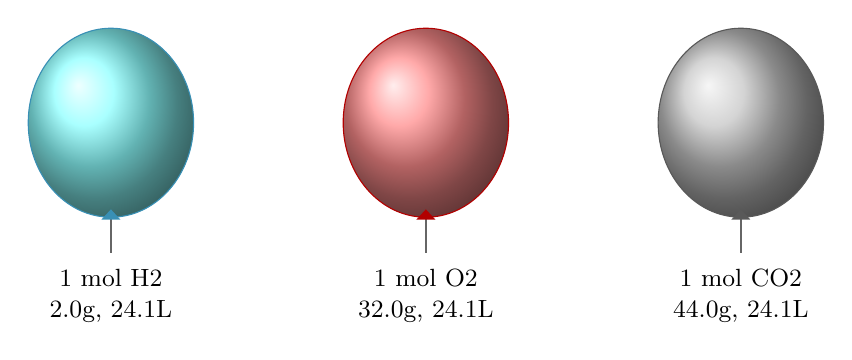
\begin{tikzpicture}[font=\small]
  \foreach \x/\g/\m/\c in {0/{\ce{H2}}/2.0/cyan, 4/{\ce{O2}}/32.0/red,
                           8/{\ce{CO2}}/44.0/gray} {
    \draw[thick, black!60] (\x,-0.25) -- (\x,-1.1);
    \shade[ball color=\c!45, draw=\c!70!black] (\x,0.55) ellipse (1.05 and 1.2);
    \fill[\c!70!black] (\x-0.12,-0.68) -- (\x+0.12,-0.68) -- (\x,-0.55) -- cycle;
    \node[align=center] at (\x,-1.65) {1 mol \g\\ \qty{\m}{g},
      \qty{24.1}{L}};
  }
\end{tikzpicture}

{\small Tiga balon pada \qty{20}{\celsius}, masing-masing berisi satu
\omterm{def:g10:the-mole:amount}{mol} gas yang berbeda. Volumenya sama; massanya tidak.}
\end{omfigure}


\begin{example}[Sebuah balon karbon dioksida]\label{ex:g10:the-mole:balloon}
% ledger: aw:C, aw:O
Sebuah balon berisi \qty{2.4}{L} karbon dioksida pada \qty{20}{\celsius}.
\omterm{def:g10:the-mole:amount}{Jumlah zatnya} $n = \qty{2.4}{L} / \qty{24.1}{L/mol} = \qty{0.10}{mol}$,
dan massanya $m = \qty{0.10}{mol} \times \qty{44.0}{g/mol} =
\qty{4.4}{g}$. Balon yang sama jika diisi hidrogen akan berisi
\qty{0.10}{mol} yang sama, tetapi hanya \qty{0.20}{g} gas.
\end{example}

\begin{remark}[Gas yang berat dan gas yang ringan]\label{rem:g10:the-mole:heavy}
Karena seliter gas apa pun mengandung \omterm{def:g10:the-mole:amount}{jumlah zat} yang sama, massa
seliter gas sebanding dengan \omterm{def:g10:the-mole:molar-mass}{massa molarnya}. \omterm{def:g4:air-a-mixture-of-gases:air}{Udara}, \omterm{def:g6:pure-substances-and-mixtures:mixture}{campuran} sekitar
empat perlima nitrogen (\qty{28.0}{g/mol}) dan seperlima oksigen
(\qty{32.0}{g/mol}), berperilaku seperti gas dengan \omterm{def:g10:the-mole:molar-mass}{massa molar} sekitar
\qty{29}{g/mol}. Gas yang \omterm{def:g10:the-mole:molar-mass}{massa molarnya} lebih besar, seperti karbon
dioksida (\qty{44.0}{g/mol}), lebih rapat daripada \omterm{def:g4:air-a-mixture-of-gases:air}{udara} dan berkumpul di
dasar gudang bawah tanah yang tertutup; gas yang \omterm{def:g10:the-mole:molar-mass}{massa molarnya} lebih
kecil, seperti helium (\qty{4.0}{g/mol}), naik.
\end{remark}

\section{Latihan}

\begin{exercise}[$\star$]\label{exo:g10:the-mole:1}
Hitung \omterm{def:g10:the-mole:molar-mass}{massa molar} gas oksigen \ce{O2}, gas nitrogen \ce{N2}, metana
\ce{CH4}, amonia \ce{NH3}, dan karbon dioksida \ce{CO2}.
\end{exercise}

\begin{exercise}[$\star$]\label{exo:g10:the-mole:2}
Berapa \omterm{def:g10:the-mole:amount}{jumlah zat} yang terkandung dalam \qty{36.0}{g} air? Dalam
\qty{4.0}{g} metana?
\end{exercise}

\begin{exercise}[$\star$]\label{exo:g10:the-mole:3}
Berapa massa \qty{0.25}{mol} natrium klorida \ce{NaCl}? Massa
\qty{2.0}{mol} karbon dioksida?
\end{exercise}

\begin{exercise}[$\star$]\label{exo:g10:the-mole:4}
Berapa \omterm{def:g7:atoms-and-molecules:molecule}{molekul} yang ada dalam \qty{0.50}{mol} gas oksigen? Berapa \omterm{def:g10:the-mole:amount}{jumlah
zat} besi yang mengandung \num{3.0e24} \omterm{def:g7:atoms-and-molecules:atom}{atom} besi?
\end{exercise}

\begin{exercise}[$\star$]\label{exo:g10:the-mole:5}
Pada \qty{20}{\celsius} dan tekanan atmosfer normal, berapa volume yang
ditempati \qty{0.50}{mol} gas nitrogen? Berapa \omterm{def:g10:the-mole:amount}{jumlah zat} gas oksigen
dalam \qty{12}{L} gas itu?
\end{exercise}

\begin{exercise}[$\star\star$]\label{exo:g10:the-mole:6}
Setetes air bervolume \qty{0.050}{mL}, dan \qty{1}{mL} air bermassa
\qty{1.0}{g}. Berapa \omterm{def:g7:atoms-and-molecules:molecule}{molekul} air yang dikandung tetes itu?
\end{exercise}

\begin{exercise}[$\star\star$]\label{exo:g10:the-mole:7}
Mana yang mengandung lebih banyak \omterm{def:g7:atoms-and-molecules:atom}{atom}, \qty{10}{g} aluminium atau
\qty{10}{g} besi? Jelaskan tanpa menghitung terlebih dahulu, lalu
periksalah dengan menghitung.
\end{exercise}

\begin{exercise}[$\star\star$]\label{exo:g10:the-mole:8}
Pada \qty{20}{\celsius}, hitung massa satu liter karbon dioksida dan
satu liter gas nitrogen. Mengapa karbon dioksida berkumpul di dasar
gudang bawah tanah tertutup tempat sari anggur sedang berfermentasi?
\end{exercise}

\begin{exercise}[$\star\star$]\label{exo:g10:the-mole:9}
Dengan gambar tiga kotak $m$, $n$, $N$, tentukan massa \num{1.0e22}
\omterm{def:g7:atoms-and-molecules:molecule}{molekul} glukosa \ce{C6H12O6}. Tuliskan kedua anak panah yang diikuti.
\end{exercise}

\begin{exercise}[$\star\star$]\label{exo:g10:the-mole:10}
Sebutir gula batu (sukrosa, \ce{C12H22O11}) bermassa \qty{5.0}{g}.
Hitung jumlah sukrosa yang dikandungnya, lalu banyaknya \omterm{def:g7:atoms-and-molecules:molecule}{molekul}
sukrosa, lalu banyaknya \omterm{def:g7:atoms-and-molecules:atom}{atom} karbon.
\end{exercise}

\begin{exercise}[$\star\star$]\label{exo:g10:the-mole:11}
Mana yang mengandung jumlah \omterm{def:g7:atoms-and-molecules:molecule}{molekul} lebih besar: \qty{1.0}{kg} air
\ce{H2O} atau \qty{1.0}{kg} etanol \ce{C2H6O}? Berapa kali lipat?
\end{exercise}

\begin{exercise}[$\star\star\star$]\label{exo:g10:the-mole:12}
Sebentuk cincin emas bermassa \qty{5.0}{g}; tiga perempat massanya
adalah emas, sisanya tembaga. Berapa \omterm{def:g7:atoms-and-molecules:atom}{atom} emas yang dikandungnya? Berapa
\omterm{def:g7:atoms-and-molecules:atom}{atom} tembaga? \omterm{def:g9:periodic-table-first-look:metal}{Logam} mana yang \omterm{def:g7:atoms-and-molecules:atom}{atomnya} lebih banyak dalam cincin itu?
\end{exercise}

\begin{exercise}[$\star\star\star$]\label{exo:g10:the-mole:13}
Sebuah ruang kelas berukuran \qty{8.0}{m} kali \qty{6.0}{m} kali
\qty{3.0}{m}, dan \omterm{def:g4:air-a-mixture-of-gases:air}{udara} di dalamnya bersuhu \qty{20}{\celsius}.
\begin{enumerate}
  \item Berapa \omterm{def:g10:the-mole:amount}{jumlah zat} gas yang dikandungnya ($\qty{1}{m^3} =
        \qty{1000}{L}$)? Berapa \omterm{def:g7:atoms-and-molecules:molecule}{molekul}?
  \item Dengan menganggap \omterm{def:g4:air-a-mixture-of-gases:air}{udara} terdiri atas 78 \omterm{def:g7:atoms-and-molecules:molecule}{molekul} gas nitrogen, 21
        \omterm{def:g7:atoms-and-molecules:molecule}{molekul} gas oksigen, dan 1 \omterm{def:g7:atoms-and-molecules:atom}{atom} argon (\qty{40.0}{g/mol}) dalam
        setiap seratus partikel, hitung \omterm{def:g10:the-mole:molar-mass}{massa molar} rata-rata \omterm{def:g4:air-a-mixture-of-gases:air}{udara}.
  \item Berapa massa \omterm{def:g4:air-a-mixture-of-gases:air}{udara} di dalam ruangan itu?
\end{enumerate}
\end{exercise}

\begin{exercise}[$\star\star\star$]\label{exo:g10:the-mole:14}
Sebuah bola silikon murni bermassa tepat \qty{1.000}{kg}.
\begin{enumerate}
  \item Berapa \omterm{def:g7:atoms-and-molecules:atom}{atom} silikon yang dikandungnya?
  \item Simpulkan massa satu \omterm{def:g7:atoms-and-molecules:atom}{atom} silikon.
  \item Sebelum 2019, \omterm{def:g10:the-mole:avogadro}{tetapan Avogadro} tidak ditetapkan tetapi diukur.
        Jelaskan bagaimana penghitungan \omterm{def:g7:atoms-and-molecules:atom}{atom} bola seperti itu secara
        terpisah, sementara \omterm{def:g10:the-mole:amount}{jumlah zatnya} diketahui dari massanya, dapat
        memberikan nilai tetapan itu.
\end{enumerate}
\end{exercise}

\begin{exercise}[$\star\star\star$]\label{exo:g10:the-mole:15}
% ledger: iso:Cl35, iso:Cl37
Klorin alami mengandung \qty{75.8}{\percent} \omterm{def:g7:atoms-and-molecules:atom}{atom} klorin-35, dengan
\omterm{def:g10:the-mole:molar-mass}{massa molar} yang sangat dekat dengan \qty{35.0}{g/mol}, dan
\qty{24.2}{\percent} \omterm{def:g7:atoms-and-molecules:atom}{atom} klorin-37, dengan \omterm{def:g10:the-mole:molar-mass}{massa molar} yang sangat dekat
dengan \qty{37.0}{g/mol}. Hitung \omterm{def:g10:the-mole:molar-mass}{massa molar atom} klorin alami, lalu
bandingkan dengan nilai pada tabel.
\end{exercise}

\section{Soal: Segelas Air Kelvin}

\begin{problem}[{Soal akhir pekan --- tuangkan segelas air ke laut,
tunggulah sampai air itu bercampur ke seluruh samudra, lalu isi gelas
itu lagi: berapa molekul dari gelas pertama yang kembali?}]
\label{pb:g10:the-mole:1}
% ledger: ocean:volume, rho:water, const:NA, aw:H, aw:O
Sebuah eksperimen pikiran yang terkenal, yang sering dikaitkan dengan
fisikawan Lord Kelvin, berbunyi seperti ini. Tandailah setiap \omterm{def:g7:atoms-and-molecules:molecule}{molekul}
dalam segelas air, tuangkan gelas itu ke laut, lalu tunggulah sampai
\omterm{def:g7:atoms-and-molecules:molecule}{molekul-molekul} yang ditandai itu tersebar merata ke seluruh samudra di
dunia. Kemudian celupkan gelas itu lagi ke laut, di mana saja. Akankah
gelas itu membawa kembali \omterm{def:g7:atoms-and-molecules:molecule}{molekul} yang ditandai? Gelas itu berisi
\qty{250}{mL}, dan \qty{1}{mL} air bermassa \qty{1.0}{g}. Samudra-samudra
berisi sekitar \qty{1.335e9}{km^3} air. Anggaplah air laut sebagai air
murni untuk penghitungan ini.

\medskip
\noindent\textbf{Bagian I --- Air di dalam gelas.}
\begin{enumerate}
  \item Hitung \omterm{def:g10:the-mole:molar-mass}{massa molar} air.
  \item Berapa massa air di dalam gelas itu?
  \item Hitung \omterm{def:g10:the-mole:amount}{jumlah zat} \omterm{def:g7:atoms-and-molecules:molecule}{molekul} air di dalam gelas itu.
  \item Berapa \omterm{def:g10:the-mole:amount}{jumlah zat} \omterm{def:g7:atoms-and-molecules:atom}{atom} hidrogen yang dikandung gelas itu? \omterm{def:g7:atoms-and-molecules:atom}{Atom}
        oksigen?
\end{enumerate}

\medskip
\noindent\textbf{Bagian II --- \omterm{def:g7:atoms-and-molecules:molecule}{Molekul} di dalam gelas.}
\begin{enumerate}[resume]
  \item Berapa \omterm{def:g7:atoms-and-molecules:molecule}{molekul} air yang dimuat gelas itu?
  \item Hitung massa satu \omterm{def:g7:atoms-and-molecules:molecule}{molekul} air, dalam gram.
  \item Periksalah jawaban soal 5 dan 6 dengan mengalikannya: berapa
        seharusnya hasil kalinya?
  \item Jika menghitung satu \omterm{def:g7:atoms-and-molecules:molecule}{molekul} per detik, siang dan malam, berapa
        tahun yang diperlukan untuk menghitung \omterm{def:g7:atoms-and-molecules:molecule}{molekul-molekul} gelas itu?
        (Satu tahun lamanya sekitar \qty{3.16e7}{s}.)
\end{enumerate}

\medskip
\noindent\textbf{Bagian III --- Samudra.}
\begin{enumerate}[resume]
  \item Ubahlah volume samudra ke dalam meter kubik
        ($\qty{1}{km^3} = \qty{e9}{m^3}$), lalu ke dalam liter.
  \item Setelah \omterm{def:g7:atoms-and-molecules:molecule}{molekul-molekul} yang ditandai tersebar merata, berapa
        banyak \omterm{def:g7:atoms-and-molecules:molecule}{molekul} itu dalam setiap liter air samudra?
  \item Berapa \omterm{def:g7:atoms-and-molecules:molecule}{molekul} yang ditandai yang dibawa kembali oleh gelas
        kedua?
  \item Cara kedua. Hitung \omterm{def:g10:the-mole:amount}{jumlah zat} air di samudra, dengan mengambil
        \qty{1.0}{kg} sebagai massa satu liter.
  \item Berapa bagian dari seluruh \omterm{def:g7:atoms-and-molecules:molecule}{molekul} air samudra yang ditandai?
  \item Kalikan bagian ini dengan banyaknya \omterm{def:g7:atoms-and-molecules:molecule}{molekul} dalam gelas kedua,
        lalu bandingkan dengan jawaban soal 11.
\end{enumerate}

\medskip
\noindent\textbf{Bagian IV --- Maknanya.}
\begin{enumerate}[resume]
  \item Berapa gelas \qty{250}{mL} yang dapat diisi dengan air
        samudra?
  \item Bandingkan bilangan ini dengan banyaknya \omterm{def:g7:atoms-and-molecules:molecule}{molekul} dalam satu
        gelas. Jelaskan dalam satu kalimat mengapa gelas kedua membawa
        kembali begitu banyak \omterm{def:g7:atoms-and-molecules:molecule}{molekul} yang ditandai.
  \item Berapa volume air laut yang harus diambil, rata-rata, untuk
        membawa kembali satu \omterm{def:g7:atoms-and-molecules:molecule}{molekul} yang ditandai? Bandingkan dengan
        setetes air \qty{0.05}{mL}.
  \item Jawaban soal 11 memiliki banyak angka. Mengapa jawaban itu
        sebaiknya hanya diberikan sebagai orde besar? Berikan dua alasan.
  \item Nyatakan jawaban akhirnya: kira-kira berapa \omterm{def:g7:atoms-and-molecules:molecule}{molekul} dari gelas
        pertama yang kembali dalam gelas kedua?
\end{enumerate}
\end{problem}
